\section{Introduction}
\label{sec:intro}

Integrated Development Environments (IDEs) are indispensable tools in the realm of software development, providing developers with a centralized platform to craft, refine, and deploy their code efficiently. These environments offer a rich array of features and utilities designed to streamline the development process, making them indispensable assets for programmers across various domains. Within the framework of an IDE, the programming assistant stands out as a crucial component, offering invaluable support to developers as they navigate the intricacies of coding. This assistant acts as a guiding hand, offering suggestions, automating repetitive tasks, and providing real-time feedback to enhance productivity and code quality.

At the heart of programming assistant tools lie sophisticated program analysis techniques. By delving deep into the structure and semantics of code, these techniques empower the assistant to offer intelligent insights and recommendations to developers. Whether it's code completion, syntax highlighting, or error detection, program analysis forms the bedrock upon which the programming assistant operates, ensuring that developers can write code with confidence and precision.

Among them, {\em the programming assistant tools that rely on
understanding a program's behaviors at runtime} play a crucial role in
assisting developers with debugging, performance optimization,
security analysis, runtime error detection, etc. By providing insights
into how a program behaves while running, these tools empower
developers to write more reliable, efficient, and secure code. First,
{\em debuggers} are essential programming assistant tools used by
developers to identify and resolve issues in their code. They allow
developers to pause the execution of a program, inspect variables and
memory, and step through code line by line. By understanding the
runtime behavior, debuggers help developers diagnose and fix bugs more
efficiently. Second, {\em dynamic analysis tools}, such as dynamic
taint analysis and dynamic symbolic execution, analyze a program's
behavior during execution to detect security vulnerabilities, such as
buffer overflows, injection attacks, and data leaks. These tools track
the flow of data and control within the program and identify potential
security threats in real-time, helping developers write more secure
code. Finally, {\em runtime error detection tools} monitor a program's
execution for runtime errors, such as null pointer dereferences,
division by zero, and out-of-bounds memory accesses. By detecting
these errors as they occur during runtime, these tools help developers
identify and fix potential issues before they manifest into serious
bugs or crashes.

However, the journey of program analysis or dynamic program's
behaviors is not without its challenges, especially when dealing with
code under editing. The {\em incompleteness and inexecutability of
code fragments} present large obstacles, making it difficult for
analysis tools to provide accurate assessments and
suggestions. Moreover, the lack of contextual information further
complicates matters, as program analysis may struggle to discern the
broader project landscape and dependencies. Another significant
challenge stems from the absence of a comprehensive {\em global
context} for program analysis within {\em the current
project}. Without access to the complete picture of the codebase and
program dependencies, analysis tools may struggle to provide nuanced
and accurate suggestions, hindering the effectiveness of the
programming assistant.

On the other hand, using {\em static analysis techniques to analyze
runtime program behaviors} has several disadvantages. Firstly, static
analysis operates solely on the source code without executing it,
which means that it tends to overestimate the dynamic behavior of the
program as it runs. This limitation makes it challenging to identify
certain runtime-specific errors or issues due to {\em the inexecutability
of incomplete code}. Moreover, static analysis may produce false
positives or false negatives, leading to inaccuracies.

Conducting runtime program analysis for incomplete and inexecutable
code during the editing phase poses challenges and
limitations. The lack of completeness and executability impedes the
ability of runtime analysis tools to accurately predict program
behavior and provide meaningful insights to developers.  When code is
incomplete, lacking crucial elements such as function definitions,
variable declarations, or control flow structures, conducting runtime
analysis becomes inherently difficult. Without a complete
understanding of the code's structure and functionality, runtime
analysis tools struggle to predict how the program would behave when
executed. Specifically, inexecutable code—code that contains missing
dependencies, or import or variable declarations presents another
obstacle to runtime analysis. Since inexecutable code cannot be
executed due to these errors, runtime analysis tools are unable to
observe the program's behavior firsthand. As a result, they cannot
gather runtime data or insights to inform their analysis.
%
Furthermore, even if runtime analysis tools attempt to analyze
incomplete or inexecutable code, their findings may be unreliable or
inaccurate. The absence of essential program elements can lead to
erroneous conclusions or misleading feedback from the analysis
tools. This can potentially misguide developers in their coding
decisions and hinder the overall development process.

It is desirable to have an approach that can strike a balance and
obtain the best of both worlds of static and dynamic analysis for
incomplete code. To this effect, we propose a novel paradigm called
{\bf predictive program analysis}, which aims to learn to analyze
program behaviors without actual program execution.

%This is enabled via the learning of semantic and execution behaviors
%of programs obtained from ultra-large-scale, open-source software
%repositories.





\subsection{Research Objectives and Anticipated Results}

\begin{figure}[t]
    \centering
    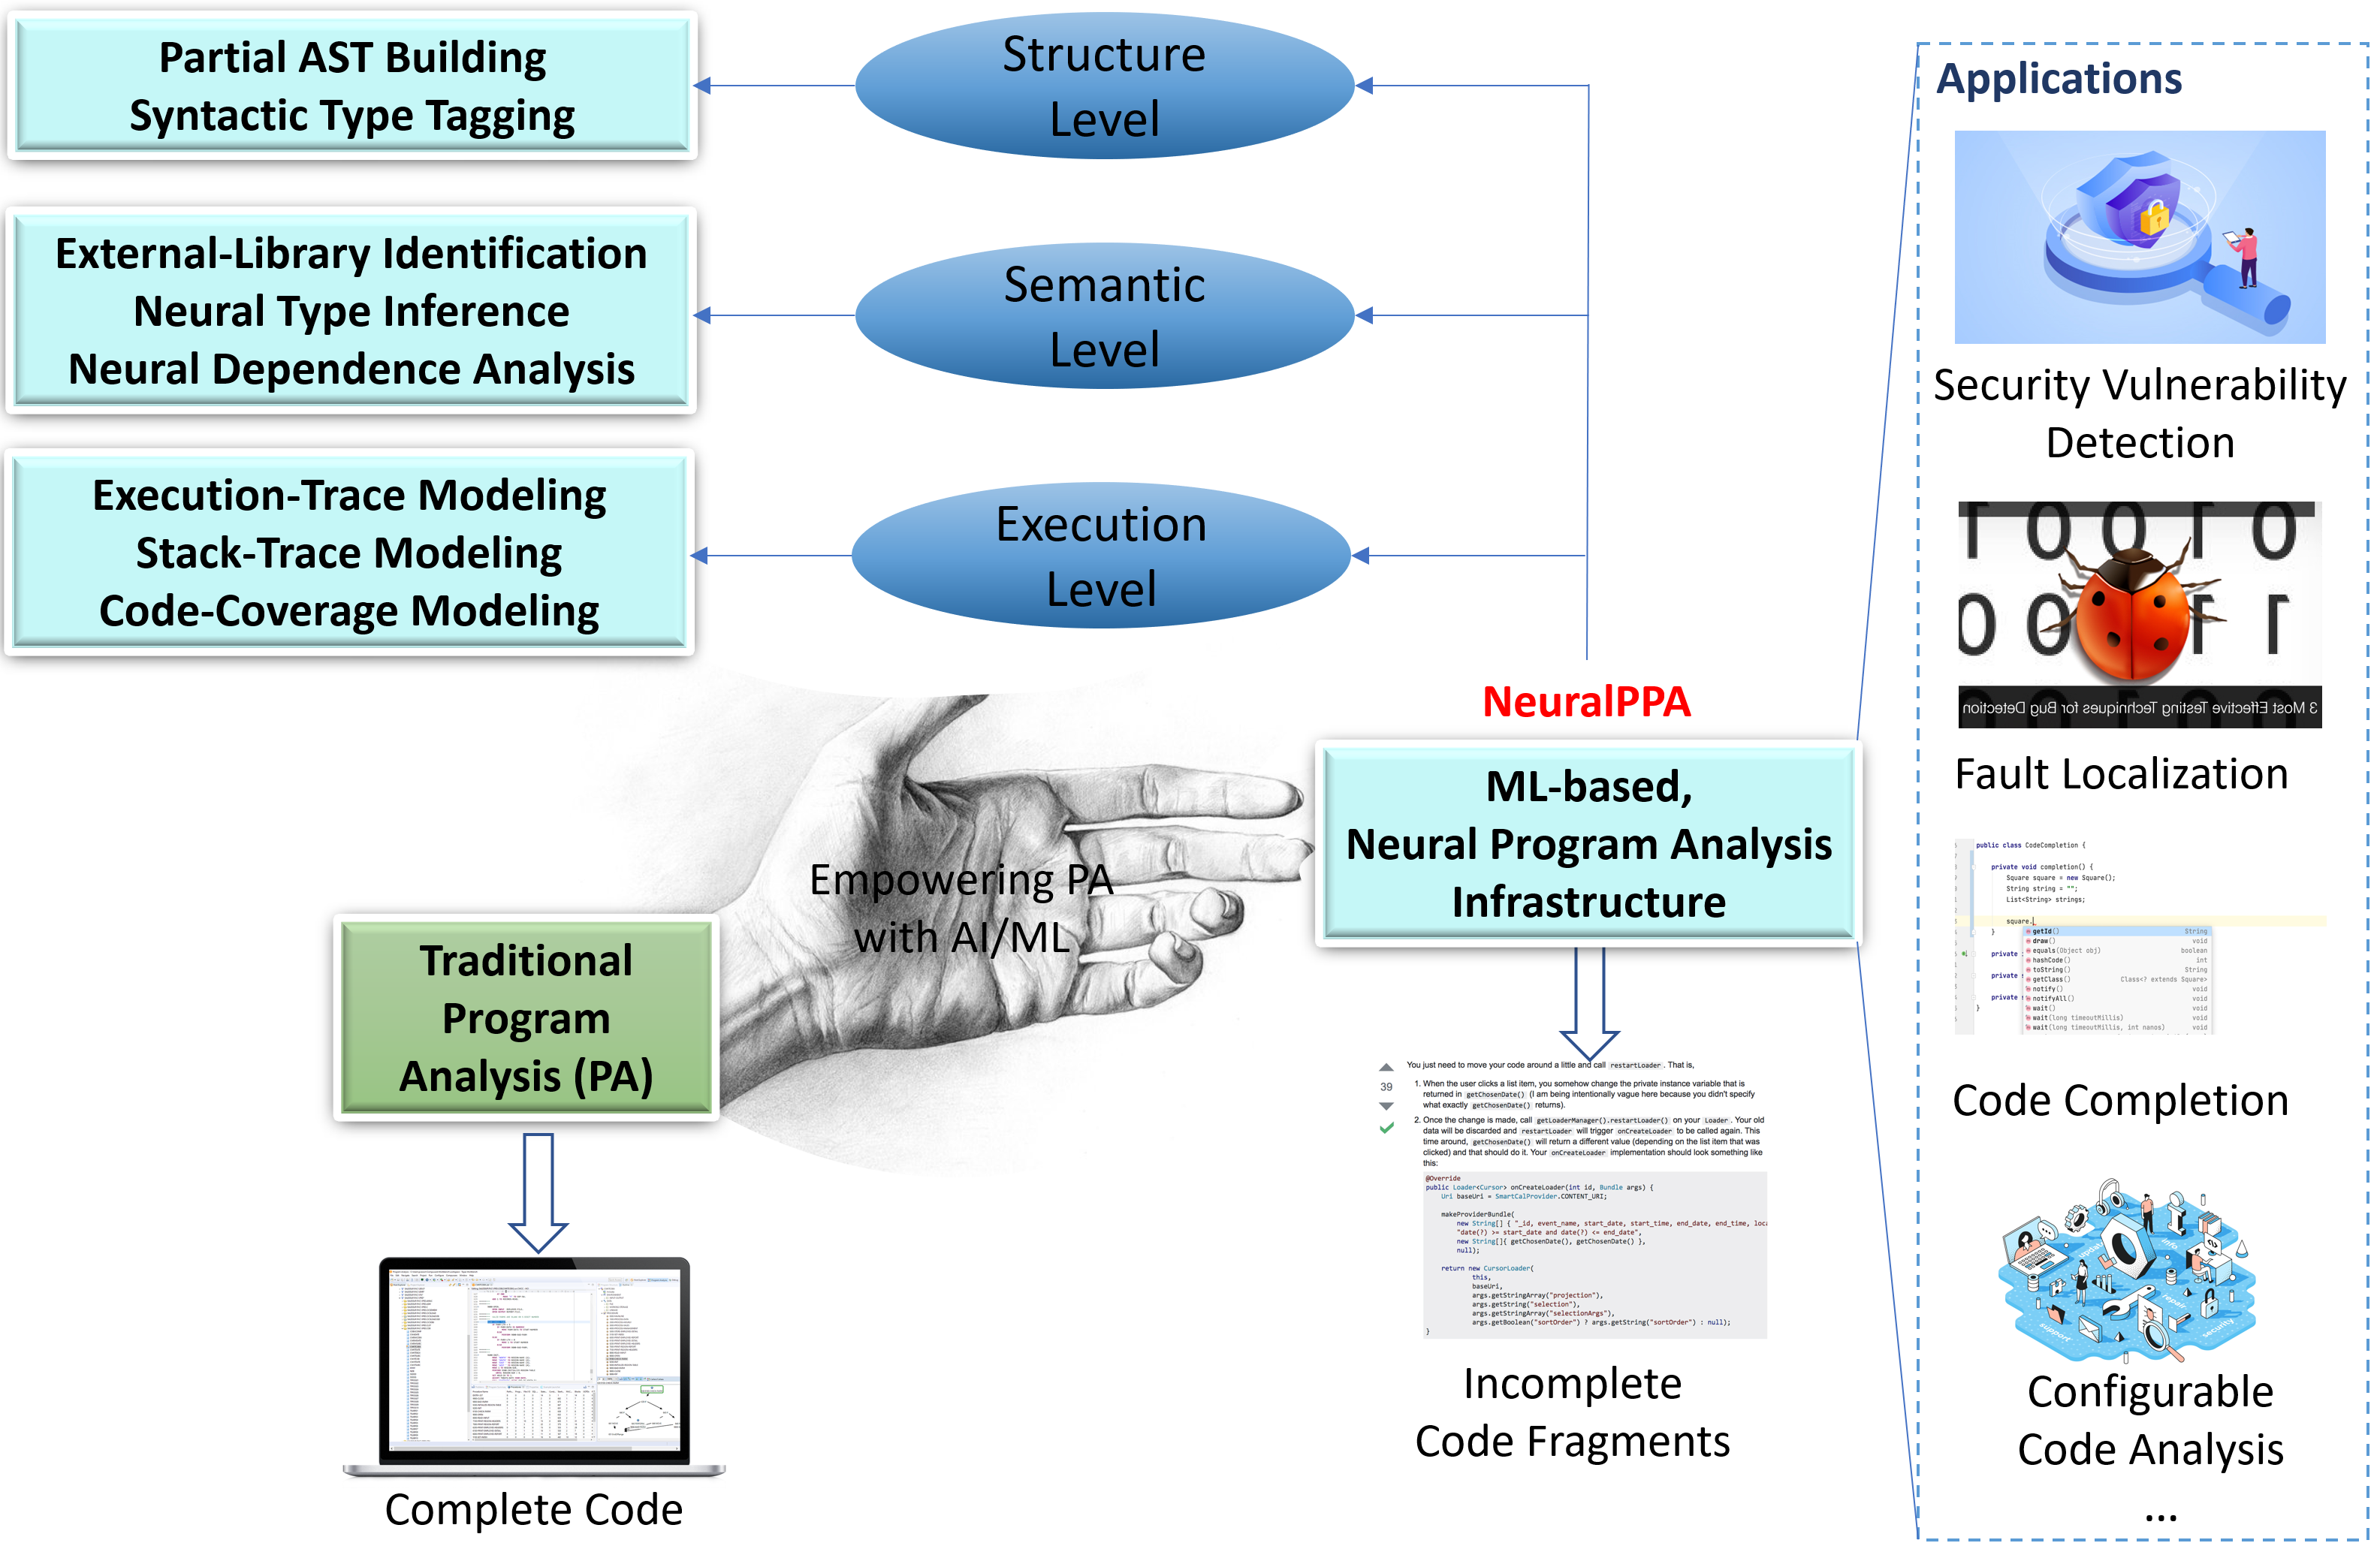
\includegraphics[width=0.9\textwidth]{graphs/neuralppa}
    \vspace{-12pt}
    \caption{{\tool}: Machine Learning-based Program Analysis Infrastructure}
    \label{fig:arch}
\end{figure}


While the state-of-the-art research and practice has been
well-established for the analysis of the entire programs, very little
research and knowledge has been achieved for partial program
analysis.
%
In this proposal, we set out to investigate and develop {\tool}, a
{\em \underline{Neural}-network-based \underline{P}artial
  \underline{P}rogram \underline{A}nalysis infrastructure}. We aim to
develop {\bf a scientific foundation, novel methodologies, frameworks,
  models, and algorithmic solutions for neural partial program
  analysis}. {\tool} {\bf enpowers program analysis (PA) with advanced
machine learning (ML) and artificial intelligence (AI) to enable the
program analysis on incomplete code fragments} (Figure~\ref{fig:arch}).
{\tool} will allow the constructions of the program analysis
techniques for partial code on which downstream software
engineering applications can be built.


In this work, our key philosophy is that {\em the analysis of
  partial code can be learned from the analysis of entire programs in
  the wealth of information from ultra-large-scale, open-source
  software repositories}.



Specifically, we draw our motivation for such a data-driven,
learning-based approach from the following. First, ultra-large-scale
software repositories, e.g. GitHub (7M+ projects) and SourceForge
(700k+ projects) contain an enormous collection of programs. These
repositories amount to 1,000,000,000+ lines of code, 10,000,000+
revision logs, and 3,000,000+ issue reports. This wealth of knowledge
is an excellent source for {\tool}. Hindle {\em et
  al.}~\cite{naturalness-icse12} have shown that code has high
repetitiveness and predictability, and can be captured well by
statistical models. Thus, we expect to build ML models to learn from
those repositories. Second, in an empirical study on the
repetitiveness, containment, and composability of PDGs in open-source
projects, the PI group~\cite{msr16} reported that among
17.5M PDGs with 1.6B PDG subgraphs, 14.3\% of the PDGs have all of
their subgraphs repeated across different projects. Furthermore, in
15.6\% of the PDGs, at least 90\% of their subgraphs are likely to
have appeared before in other projects. Thus, {\tool} could learn from
PDGs with complete program dependencies retrieved from existing code
repositories and derive the dependencies for the (partial) code
fragment under study. The PI group also reported a high repetitiveness
level for AST code structure in open-source
projects~\cite{icse15}. Finally, such a program analysis
infrastructure like {\tool} can be drawn from the spirit and successes
of the approaches in natural language processing (NLP). For example,
at the lexical level, the task of deriving the token types for source
code tokens could be analogous to the part-of-speech (PoS) tagging in
NLP. At the syntax level, the task of learning the syntactic structure
in AST of the partial code can be inspired by the approaches to build
parse trees for natural-language texts. At the semantic level, the
partial program dependence analysis infrastructure is similar in
spirit to the the neural network-based dependency parsing in NLP,
which learns the dependencies signifying the semantic relationships
between words in a sentence from text corpora.

Toward this theme, in our preliminary work, we developed DeepPDA, a neural
network-based partial program dependence analysis approach that learns
to derive the program dependencies for any code fragments (i.e., both
complete and incomplete). In our preliminary empirical evaluation, we
intrinsically evaluated it on Java and C/C++ programs. First, we
trained {\tool} on complete code. For testing, we treated each method
individually and chose a consecutive portion within the method to
predict the program dependencies, and compared them against the actual
dependencies. Overall, DeepPDA predicts CFG and PDG edges in Java
with an F-score of 94.29\%, and in C++ with an F-score of
92.46\%.
%
We also developed as an approach to derive the data
types of the variables in the code snippets. We treat the problem as
statistical machine translation from source code with partially
qualified names to source code with FQNs of the APIs. Our empirical
evaluation on real-world code and StackOverflow posts shows that our
technique achieves high accuracy with 97.6\% precision and 96.7\%
recall in deriving data types in code snippets.


In {\tool}, we propose the following thrusts of research
(Table~\ref{tab:milestones}):

\vspace{3pt}
\noindent \textbf{Thurst 1. Neural Structural Analysis Infrastructure
  \code{NeuralStruct}.} ({\em Section~\ref{}}) Source code has
well-defined structures and semantics. Thus, the basic infrastructure
in {\tool} is the neural structural analysis (\code{NeuralStruct})
component.  This component has two main tasks. First, it learns from
the syntactic structures of the complete code in the training dataset
collected from large-scale code repositories, to derive the abstract
syntax tree (AST) that best represents the syntactic structure of the
given partial code, i.e., with the highest likelihood/probability.
The traditional lexical analyzer still works for partial code due to
the independence nature of lexical tokens. The second task of this
component is to tag the code tokens with the types of the syntactic
units including the statement types (\code{if}, \code{for}, etc.),
variables, fields, methods, classes, etc. Both of the tasks can be
performed with our learning-based approaches in a dual-learning
manner.
  
\vspace{3pt}
\noindent \textbf{Thurst 2. Neural Semantic Analysis Infrastructure.}
({\em Section~\ref{}}) The basis components for several program
analysis techniques include the following:

1) the identification of the APIs of the external libraries in the
external references in the partial code: this is needed because the
partial code contains the undeclared reference and/or
declaration/reference ambiguity without explicit declaration of the
APIs in the external libraries.

2) the inference of the type information for the entities in the
partial code: due to the ambiguity in the declaration, the types of
the variables and statements are not always obviously defined. Thus,
the type inference is a basic service within {\tool}.

3) the inference of the program dependencies among the statements in
the partial code: several program analysis techniques are based on the
program dependencies, which are not always obtainable due to the
incompleteness of the given code fragment.

\vspace{3pt}
\noindent \textbf{Thurst 3. Neural Symbolic Execution Infrastructure.}
...

\vspace{3pt}
\noindent \textbf{Thurst 4. Neural Partial Program Analysis
  Applications.}  ({\em Section~\ref{}}) Our last thrust of research
is aimed to evaluate our basic partial program analysis infrastructure
in a few applications. We choose the following software engineering
applications: 1) software vulnerability detection for code snippets,
2) fault localization, and 3) code completion.

\vspace{3pt}
\noindent \textbf{Thurst ???. Neural Execution Analysis Infrastructure.}
({\em Section~\ref{}}) All the dynamic analysis techniques require the
analysis and understanding of the execution. However, for an
incomplete code, we first need to design a component that can wrap
around the given code fragment with the minimum code so that the code
fragment can be executed. When the code is executed, we also need the
approaches that represent the executed statements and their relations,
model the execution and stack traces, and model the code coverages
for an execution.


\begin{table*}[t]
	\vspace{-15pt}
\begin{center}
{\footnotesize{
\begin{tabular}{cc}
\begin{tabular}[t]{|p{0.2in}|p{2.95in}|} 
\hline
\multicolumn{2}{|>{\columncolor[gray]{0}}c|}{\textcolor{white}
{\bf Year 1 Project Milestones \& Deliverables}}\\
\hline 
\hline
\multicolumn{2}{|c|}{\bf T1. Neural Structure Analysis Infrastructure}\\
\hline
{\bf 1.1} & Neural Syntactic Type Tagging\\
{\bf 1.2} & Neural Partial AST Building\\
{\bf 1.3} & Evaluation of the components\\
\hline
\hline
\multicolumn{2}{|c|}{\bf T2. Neural Semantic Analysis Infrastructure}\\ 
\hline
{\bf 2.1} & External-Library Identification\\
\hline
%\hline
%\multicolumn{2}{|c|}{\bf Integrate Code Synthesis into Tools}\\
%\hline
%{\bf 1.5} & \goalOneFour.\\
%\hline
\multicolumn{2}{c}{}
\end{tabular}
&
\begin{tabular}[t]{|p{0.2in}|p{2.95in}|} \hline
\multicolumn{2}{|>{\columncolor[gray]{0}}c|}{\textcolor{white}
{\bf Year 2 Project Milestones \& Deliverables}}\\
\hline 
\hline
\multicolumn{2}{|c|}{\bf T2. Neural Semantic Analysis Infrastructure}\\
\hline
{\bf 2.2} & Neural Type Inference\\
{\bf 2.3} & Neural Dependence Analysis\\
%{\bf 2.3} & Integrate Evaluation Framework into Design Environment\\
%{\bf 2.4} & Evaluate CRL Framework with Existing Models\\
%{\bf 2.3} & \goalTwoThree.\\

\hline
\hline
\multicolumn{2}{|c|}{\bf T3. Neural Execution Analysis}\\ 
\hline
%{\bf 3.1} & Design New Code Representations and Learning Models.\\
{\bf 3.1} & Neural Execution-Trace Modeling\\
%{\bf 2.4} & Advance FL and RT-CI Approaches.\\
%{\bf 2.5} & Advance Regression Testing in CI Approaches.\\
%{\bf 2.5} & Advance APR Approaches with Framework.\\
\hline
%\hline
%\multicolumn{2}{|c|}{\bf Community Involvement: Capacity Building}\\
%\hline
%{\bf 2.4} & \goalTwoFour.\\
%{\bf 2.5} & \goalTwoFive.\\
%{\bf 2.6} & \goalTwoSix.\\
%\hline
\multicolumn{2}{c}{}
\end{tabular}
\end{tabular}\\
\vspace*{-.3cm}
\begin{tabular}{c}\hline
\multicolumn{1}{|>{\centering\columncolor[gray]{0}}p{6.44in}|}{\textcolor{white}
{\bf Year 3 Project Milestones \& Deliverables}}\\
\hline
\end{tabular}\\
\vspace*{-.2cm}
\begin{tabular}{cc}
\begin{tabular}[t]{|p{0.2in}|p{2.95in}|}
\hline
\multicolumn{2}{|c|}{\bf T3. Neural Execution Analysis}\\
\hline
{\bf 3.2} & Neural Stack Trace Modeling\\
{\bf 3.3} & Neural Code Coverage Modeling\\

%{\bf 3.3} & Testing on Models in IDE tools.\\
\hline
%\hline
%\multicolumn{2}{|c|}{\bf \goalTwo}\\ 
%\hline
%{\bf 3.3} & \goalThreeThree.\\
%\hline
\multicolumn{2}{c}{}
\end{tabular}
&
\begin{tabular}[t]{|p{0.2in}|p{2.95in}|}
\hline
\multicolumn{2}{|c|}{\bf T4. Neural Partial Program Analysis Applications}\\
\hline
%{\bf 3.1} & Design New Code Representations\\

{\bf 4.1} & Security Vulnerablity Detection with {\tool}\\
{\bf 4.2} & Fault Localization and Completion with {\tool}\\

\hline
\multicolumn{2}{c}{}
\end{tabular}
\end{tabular}
\vspace{-15pt}
}}
\end{center}
\vspace*{-.3in}
%\caption{Tasks and Milestones. (Rep. = Representation)}
\caption{The 3-year schedule of Thrusts, Tasks, and Milestones of this proposal.}
%the schedule of Thrusts, Tasks, and Milestones of this proposal.
%\vspace{-10pt}
\label{tab:milestones}
\vspace{-10pt}
\end{table*}
%






%\subsection{Significance of This Proposed Project: NSF Merit Criteria}

\section{Relevance to Secure and Trustworthy Cyberspace}

This project will develop novel concepts, representations, algorithms,
models, and tools to support early software vulnerability
detection. It is transformative and directly help improve software
quality with novel program analysis-based software security and
vulnerability detection tools on code snippets.

\section{Intellectual Merits}

%The results of this project will be transformative and directly help
%improve software quality with novel program analysis-based software
%security tools.

\noindent \underline{{\bf Advance the state-of-the-art knowledge and
    understanding}}. Neural program analysis infrastructure in Thrusts
1--3 will advance the body of knowledge and theoretical foundations
for machine learning and AI for code. Thrust 4 will also help advance the
practical tools in software security and engineering.

\noindent \underline{{\bf Scientific foundation, creative/original
    research}}. (1) to enable the analysis on partial code, (2) to empower
the program analysis techniques on both (in)complete code,
and (3) to enable the applications of program analysis on incomplete
code such as vulnerability detection on code snippets, etc.

\section{Broader Impacts}

\underline{{\bf (1) Transformative and benefits to society}}. Our
results will be transformative and directly benefit to our society.
They will lead to increasing developers' productivity, software
quality \& reliability.  Our validation involves students and
professionals, promoting teaching, training, and learning of both {\bf
  software security} and {\bf machine learning} techniques that
have wide impacts in industry and academic communities.

\noindent\underline{{\bf (2) Foster other related research
    activities}}. Our results will foster {\em research activities in
  related fields of {\bf machine learning} and {\bf program analysis}},
and the applications in software security and reliability.
%We will produce theoretical concepts and techniques that are novel in
%deep learning, e.g., novel neural networks to model and learn for
%code.
%The applications of our neural program analysis in software
%engineering applications will advance software security and
%reliability.

%The collected {\bf large scale bug\&fix corpus} will be useful for
%software quality and reliability research.
%Innovations in CRL could be used to {\bf advance other SE tasks}. We
%will also develop {\bf novel DL-based bug detect-fix} approaches.


\noindent\underline{{\bf (3) Education, dissemination, and broader participation}} (Section~\ref{edu}). The
research will enhance the infrastructure for teaching/research via
tools and data sets for use by students and practitioners, and for
enhancement by researchers. We will provide related learning
modules for educators as well. It will include outreach activities for
undergraduate students, underrepresented groups, minorities, and women
in science.
%contribute novel
%teaching modules to our curriculum.
%Details will be presented in Section~\ref{edu}


\iffalse
\begin{itemize}
	\vspace{-5pt}
\itemsep-0.2em 
  \item {\bf Transformative and benefits to society}. Our 
    results will be transformative and directly benefit to our
    society. 
    They will lead to increasing developers' productivity
    and software quality \& reliability. 
    Our validation involves students and
    professionals, promoting teaching, training, and learning of bug detecting and fixing techniques that have wide impacts 
    in industry and academic communities.

%report

  \item {\bf Foster other research activities}. Our results will
    foster research activities in related fields of deep learning and
    software quality. 
    This project will produce theoretical
    concepts and techniques that are novel even in deep learning, e.g.,
    novel neural networks for modeling and learning code. 
    The collected large scale bug fixing corpus will be useful for software quality and reliability research in general.
    %e.g.,   code transformation. 
%    This project will also advance
%    the state-of-the-art research in large-scale program analysis with
%    deep neural network models.

%The representation for software security vulnerabili will be useful in
%research on software security, malware detection, vulnerability
%reports, and automatic security patching.


  \item {\bf Education, dissemination, and broader participation}.
  The research will enhance the infrastructure for teaching and
  research by providing tools and data sets for use by students and
  practitioners, and for enhancement by other researchers. We will
  provide related learning modules for educators as well. It will
  contribute novel teaching modules to our curriculum. Details will be
  presented in Section~\ref{edu}

%Details are in Section 4.

\end{itemize}
\fi
